\documentclass{beamer}

\usepackage[utf8x]{inputenc}
\usepackage{graphicx}
\usepackage{setspace}
\usepackage{tikz}
\usepackage{algorithm}
\usepackage{algpseudocode}
\usepackage{array}
\usepackage{amsmath}

\usetikzlibrary{arrows,decorations.pathmorphing,backgrounds,positioning,fit,petri}

\usetheme{Boadilla}
\usecolortheme{dolphin}
\usefonttheme{structurebold}

\setbeamertemplate{footline}
{
}


\title{Static Single Assignment Form}
\author{Luka Stojanović}
\institute{
  luka@magrathea.rs \\
  Seven Bridges Genomics
}
\date{Scalability\#06 \\ 23. 12. 2012.}
\subject{Computer Science}

\begin{document}
  \begin{frame}
    \titlepage
  \end{frame}
  
  \begin{frame}
    \frametitle{Outline}
    \tableofcontents
  \end{frame}
  
  \section{Introduction (What? Why?)}
  \begin{frame}
    \frametitle{What is SSA Form?}
    \begin{block}{SSA Form}
    	Property of compiler's IR, which says that each variable is assigned exactly once.
    \end{block}
    
    \begin{itemize}
    	\item Developed during 1980's and described in the paper
    \emph{Efficiently computing static single assignment form and the control dependence graph}
    by Ron Cytron , Jeanne Ferrante , Barry K. Rosen , Mark N. Wegman , F. Kenneth Zadeck from 1991.
    	\item Convenient for various optimization techniques.
    \end{itemize}
    
  \end{frame}
  
  \begin{frame}
    \frametitle{What is SSA Form}
	\begin{columns}
	\begin{column}{0.30\textwidth}
    	\begin{algorithm}[H]
    	\begin{algorithmic}
			\State $i := 0$
			\State $i := 5$
			\State $j := i$
		\end{algorithmic}
	    \end{algorithm}
	\end{column}
	
	\begin{column}{0.06\textwidth}
		$\Longrightarrow$
	\end{column}
	
	\begin{column}{0.30\textwidth}
		\begin{algorithm}[H]
		\begin{algorithmic}
			\State $i_1 := 0$
			\State $i_2 := 5$
			\State $j_1 := i_2$
		\end{algorithmic}
		\end{algorithm}
	 \end{column}
	 
	\begin{column}{0.33\textwidth}
		It becomes apparent that although $i$ is used, $i_1$ isn't, 
		and can be optimized away.
	\end{column}
	\end{columns}
	
	\begin{columns}
	\begin{column}{0.3\textwidth}
    	\begin{algorithm}[H]
    	\begin{algorithmic}
			\If {condition}
				\State $i := 0$
			\Else			
				\State $i := 5$
			\EndIf
			\State $j := f(i)$
		\end{algorithmic}
	    \end{algorithm}
	\end{column}
	
	\begin{column}{0.06\textwidth}
		$\Longrightarrow$
	\end{column}
	
	\begin{column}{0.30\textwidth}
		\begin{algorithm}[H]
		\begin{algorithmic}
			\If {condition}
				\State $i_1 := 0$
			\Else			
				\State $i_2 := 5$
			\EndIf
			\only<1-1>{\State $j_1 := f(i_?)$}
			\only<2->{\State $i_3 := \phi(i_1, i_2)$
			\State $j_1 := f(i_3)$}
		\end{algorithmic}
		\end{algorithm}
	 \end{column}
	 
	\begin{column}{0.33\textwidth}
		\only<1-1>{What value of $i$ is used in this expression?}
		\only<2->{There is an artificial instruction $\phi$ inserted to designate
			that values from multiple branches are merged at this spot.}
	\end{column}
	\end{columns}	
	
  \end{frame}

  \begin{frame}
    \frametitle{Optimizations}
    \begin{itemize}
		\item Constant propagation
		\item Value range propagation
		\item Global value numbering
		\item Strength reduction
		\item Dead code elimination
		\item Register allocation
    \end{itemize}
  \end{frame}
  
  \begin{frame}
    \frametitle{Register allocation}
    \begin{block}{Graph Coloring}
    	\emph{Graph Coloring} is a problem of coloring the vertices of a graph such that no two adjacent vertices share the same color.
    \end{block}

	Register allocation can be abstracted into graph coloring problem using these abstractions:
    \begin{itemize}
    	\item A variable corresponds to a node in an undirected graph.
    	\item If two variables are alive at the same time, their nodes are connected by an edge.
	\end{itemize}	

	Since graph coloring is NP-complete, register allocation is calculated using a heuristic.

  \end{frame}
  
  \begin{frame}
    \frametitle{Register allocation}
    \begin{columns}
       	\begin{column}{0.5\textwidth}
       		If program is in SSA form, corresponding variable graph is ,,chordial'', and problem of it's coloring becomes polynomial.
    	\end{column}
       	
    	\begin{column}{0.5\textwidth}
    	    \begin{figure}
			    \includegraphics[width=0.9\textwidth]{chordal-graph}
	    		\caption{Chordial graph}
    		\end{figure}
    	\end{column}
    \end{columns}
  \end{frame}  
  
  \section{Calculation}
  \begin{frame}
    \frametitle{Computing SSA Form}
    \begin{definition}
    	A \emph{control flow graph} is a directed graph whose nodes are the basic blocks of program, and two additional nodes \textbf{Entry} and \textbf{Exit}.
    \end{definition}
  \end{frame}

  \begin{frame}[shrink=30]
    \frametitle{Control Flow Graph}
	\begin{columns}
	\begin{column}{0.30\textwidth}
    	\begin{algorithmic}
			\State $i := 1$
			\State $j := 1$
			\State $k := 1$
			\State $l := 1$
			\Repeat
				\If {P}
					\State $j := i$
					\If {Q}
						\State $l := 2$
					\Else
						\State $l := 3$
					\EndIf
					\State $k := k + 1$
				\Else
					\State $k := k + 2$
				\EndIf
				\State $print(i, j, k, l)$
				\Repeat
					\If {R} \State $l := l + 4$
					\EndIf
				\Until {S}
				\State $i := i + 6$
			\Until {T}
					
		\end{algorithmic}
	\end{column}
	
	\begin{column}{0.18\textwidth}
		\\
		(1) \\
		(1) \\
		(1) \\
		(1) \\
		(2) \\
		(2) \\
		(3) \\
		(3) \\
		(4) \\
		(5) \\
		(5) \\
		(6) \\
		(6) \\
		(7) \\
		(7) \\
		(8) \\
		(8) \\
		(9) \\
		(9) \\
		(10) \\
		(11) \\
		(11) \\
		(12) \\
		(12)
	\end{column}

	\begin{column}{0.50\textwidth}
		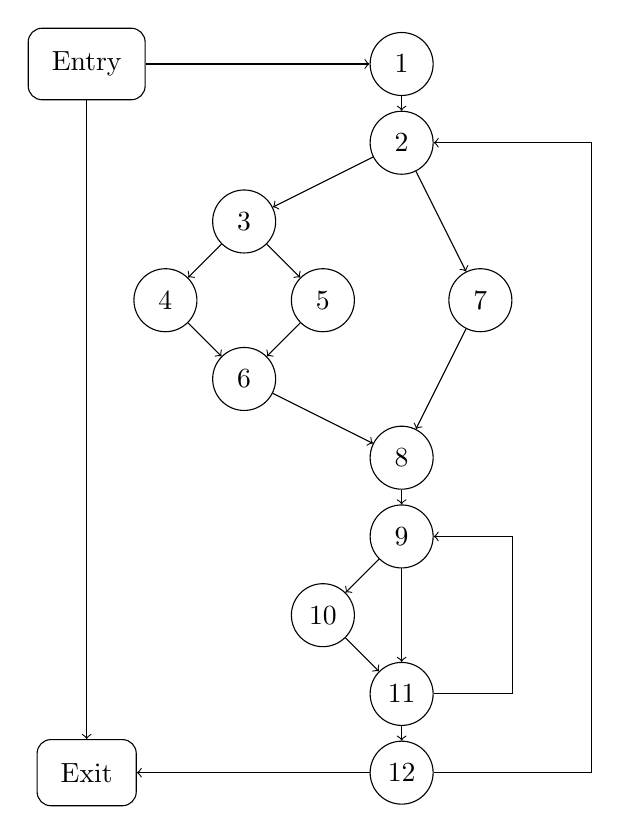
\begin{tikzpicture}[
				num/.style={draw,circle,minimum width=8mm},
				txt/.style={draw,rounded corners=5pt, inner sep=3mm}]
			\node [txt] (entry) at (0,0) {Entry};
			\node [num] (1) at (4,0) {1}
				edge[<-](entry);
			\node [num] (2) at (4,-1) {2}
				edge[<-](1);
			\node [num] (3) at (2,-2) {3}
				edge[<-](2);
			\node [num] (4) at (1,-3) {4}
				edge[<-](3);
			\node [num] (5) at (3,-3) {5}
				edge[<-](3);
			\node [num] (6) at (2,-4) {6}
				edge[<-](4)
				edge[<-](5);
			\node [num] (7) at (5,-3) {7}
				edge[<-](2);
			\node [num] (8) at (4,-5) {8}
				edge[<-](6)
				edge[<-](7);
			\node [num] (9) at (4,-6) {9}
				edge[<-](8);
			\node [num] (10) at (3,-7) {10}
				edge[<-](9);
			\node [num] (11) at (4,-8) {11}
				edge[<-](10)
				edge[<-](9);
			\node [num] (12) at (4,-9) {12}
				edge[<-](11);
			\node [txt] (exit) at (0,-9) {Exit}
				edge[<-](12)
				edge[<-](entry);
			\draw [->] (11.east) -- +(1,0) |- (9.east);
			\draw [->] (12.east) -- +(2,0) |- (2.east);
		\end{tikzpicture}
	\end{column}
	\end{columns}
  \end{frame}

\begin{frame}[shrink=50]
    \frametitle{SSA}
	\begin{columns}
	\begin{column}{0.50\textwidth}
    	\begin{algorithmic}
			\State $i := 1$
			\State $j := 1$
			\State $k := 1$
			\State $l := 1$
			\Repeat
				\\
				\\
				\\
				\\
				\If {P}
					\State $j := i$
					\If {Q}
						\State $l := 2$
					\Else
						\State $l := 3$
					\EndIf
					\\
					\State $k := k + 1$
				\Else
					\State $k := k + 2$
				\EndIf
				\\
				\\
				\\
				\State $print(i, j, k, l)$
				\Repeat
				\\
					\If {R} \State $l := l + 4$
					\EndIf
					\\
				\Until {S}
				\State $i := i + 6$
			\Until {T}
		\end{algorithmic}
	\end{column}
	
	\begin{column}{0.45\textwidth}
		\begin{algorithmic}
			\State $i_1 := 1$
			\State $j_1 := 1$
			\State $k_1 := 1$
			\State $l_1 := 1$
			\Repeat
				\State $i_2 := \phi(i_3, i_1)$
				\State $j_2 := \phi(j_4, j_1)$
				\State $k_2 := \phi(k_5, k_1)$
				\State $l_2 := \phi(l_9, l_1)$
				\If {P}
					\State $j_3 := i_2$
					\If {Q}
						\State $l_3 := 2$
					\Else
						\State $l_4 := 3$
					\EndIf
					\State $l_5 := \phi(l_3, l_4)$
					\State $k_3 := k_2 + 1$
				\Else
					\State $k_4 := k_2 + 2$
				\EndIf
				\State $j_4 := \phi(j_3, j_2)$
				\State $k_5 := \phi(k_3, k_4)$
				\State $l_6 := \phi(l_2, l_5)$
				\State $print(i_2, j_4, k_5, l_6)$
				\Repeat
					\State $l_7 := \phi(l_9, l_6)$
					\If {R} \State $l_8 := l_7 + 4$
					\EndIf
					\State $l_9 := \phi(l_8, l_7)$
				\Until {S}
				\State $i_3 := i_2 + 6$
			\Until {T}
		\end{algorithmic}
	\end{column}
	\end{columns}
  \end{frame}

  \begin{frame}
    \frametitle{Control Flow Graph}
    \begin{definition}
    	For any non-negative integer $J$, a \emph{path of length $J$}
    	consists of a sequence of $J + 1$ nodes ($X_0,\ldots,X_J$) 
    	and $J$ edges ($e_1,\ldots,e_J$).
    \end{definition}
    
    Node or edge may repeat several times within same sequence. 
    The \emph{null} path, with $J = 0$ is allowed. 
    We write 
    	$p: X_0\overset{\ast}{\rightarrow}X_J$ 
    for unrestricted path and 
    	$p: X_0\overset{+}{\rightarrow}X_J$
    for paths known to be non-null.
    
	\begin{enumerate}
	    \item If two non-null paths 
	    	$X\overset{+}{\rightarrow}Z$ and $Y\overset{+}{\rightarrow}Z$ 
	    	converge at node Z, 
	    	and nodes $X$ and $Y$ contain assignments to $V$,
	    	then $V := \phi(V,\ldots,V)$ is inserted in $Z$
	    \item Each mention of $V$ is replaced with $V_i$
	    \item For every $V$ in original program, $V_i$ in the new program must have the same value.
	\end{enumerate}    
    
  \end{frame}

  \begin{frame}
  	\frametitle{Minimal SSA Form}
  	\begin{itemize}
    	\item The \emph{dominance frontier} mapping is constructed from CFG
    	\item Using dominance frontiers, locations of $\phi$-functions is calculated
    	\item Variables are renamed
    \end{itemize}
    
	\begin{definition}
    	The \emph{dominance frontier} $DF(X)$ is the set of all CFG nodes $Y$
    	such that $X$ dominates predecessor of $Y$ 
    	but doesn't strictly dominate $Y$
    \end{definition}    
    
    \begin{definition}
    	The \emph{dominance frontier} $DF(X)$ is the set of all CFG nodes $Y$
    	such that $X$ dominates predecessor of $Y$ 
    	but doesn't strictly dominate $Y$ \\
    	$DF(X( = \lbrace Y | (\exists P \in Pred(Y)) (X \geqslant P{} and{} X \ngeqslant Y)\rbrace$
    \end{definition}
  \end{frame}

  \begin{frame}[shrink=25]
  \frametitle{Dominator Tree}
    \begin{columns}
	\begin{column}{0.45\textwidth}
		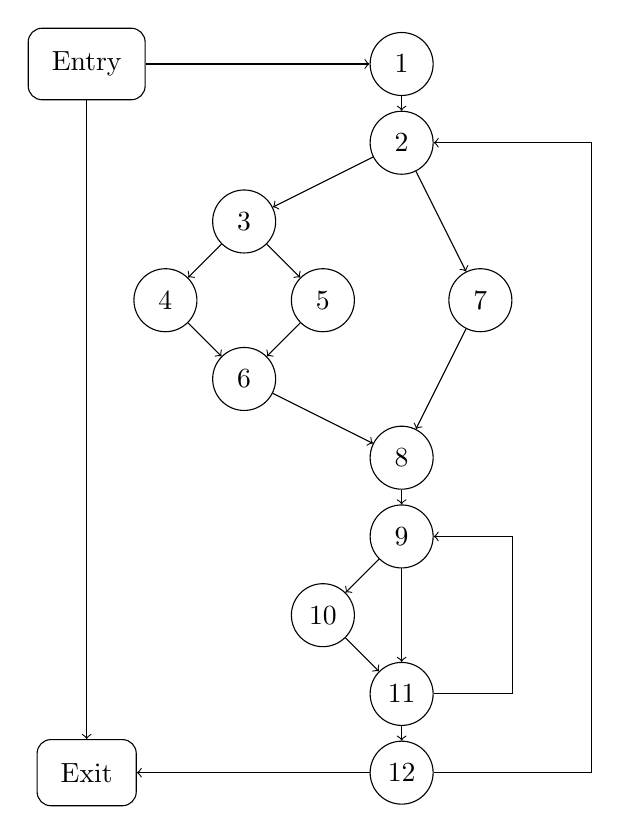
\begin{tikzpicture}[
				num/.style={draw,circle,minimum width=8mm},
				txt/.style={draw,rounded corners=5pt, inner sep=3mm}]
			\node [txt] (entry) at (0,0) {Entry};
			\node [num] (1) at (4,0) {1}
				edge[<-](entry);
			\node [num] (2) at (4,-1) {2}
				edge[<-](1);
			\node [num] (3) at (2,-2) {3}
				edge[<-](2);
			\node [num] (4) at (1,-3) {4}
				edge[<-](3);
			\node [num] (5) at (3,-3) {5}
				edge[<-](3);
			\node [num] (6) at (2,-4) {6}
				edge[<-](4)
				edge[<-](5);
			\node [num] (7) at (5,-3) {7}
				edge[<-](2);
			\node [num] (8) at (4,-5) {8}
				edge[<-](6)
				edge[<-](7);
			\node [num] (9) at (4,-6) {9}
				edge[<-](8);
			\node [num] (10) at (3,-7) {10}
				edge[<-](9);
			\node [num] (11) at (4,-8) {11}
				edge[<-](10)
				edge[<-](9);
			\node [num] (12) at (4,-9) {12}
				edge[<-](11);
			\node [txt] (exit) at (0,-9) {Exit}
				edge[<-](12)
				edge[<-](entry);
			\draw [->] (11.east) -- +(1,0) |- (9.east);
			\draw [->] (12.east) -- +(2,0) |- (2.east);
		\end{tikzpicture}
	\end{column}
	\begin{column}{0.55\textwidth}
		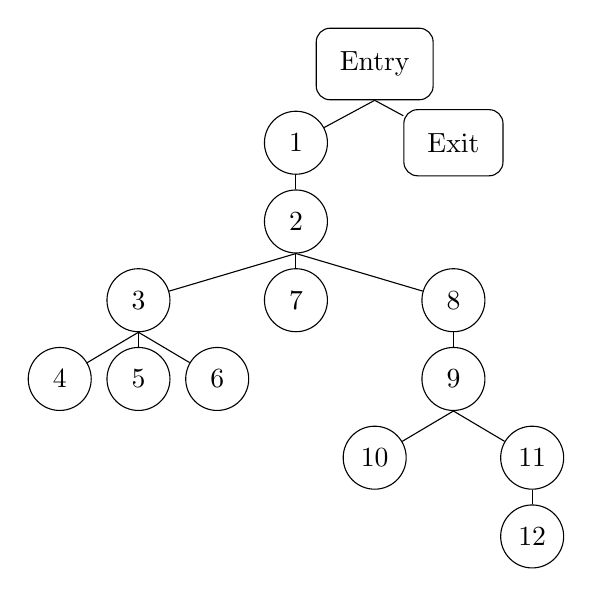
\begin{tikzpicture}[
				num/.style={draw,circle,minimum width=8mm},
				txt/.style={draw,rounded corners=5pt, inner sep=3mm}]
			\node [txt] (entry) at (4,0) {Entry};
			\node [txt] (exit) at (5,-1) {Exit}
				edge[-] (entry.south);
			\node [num] (1) at (3,-1) {1}
				edge[-] (entry.south);
			\node [num] (2) at (3,-2) {2}
				edge[-] (1.south);
			\node [num] (3) at (1,-3) {3}
				edge[-] (2.south);
			\node [num] (4) at (0,-4) {4}
				edge[-] (3.south);
			\node [num] (5) at (1,-4) {5}
				edge[-] (3.south);
			\node [num] (6) at (2,-4) {6}
				edge[-] (3.south);
			\node [num] (7) at (3,-3) {7}
				edge[-] (2.south);
			\node [num] (8) at (5,-3) {8}
				edge[-] (2.south);
			\node [num] (9) at (5,-4) {9}
				edge[-] (8.south);
			\node [num] (10) at (4,-5) {10}
				edge[-] (9.south);
			\node [num] (11) at (6,-5) {11}
				edge[-] (9.south);
			\node [num] (12) at (6,-6) {12}
				edge[-] (11.south);
		\end{tikzpicture}
	\end{column}	
	
	\end{columns}  
  \end{frame}
  
  \begin{frame}[shrink=30]
  	\frametitle{Placement of $\phi$ functions}
  	\begin{algorithmic}
  		\State $IterCount := 0$
  		\For{each node X}
  			\State $HasAlready[X] := 0$
  			\State $Work[X] := 0$
  		\EndFor
  		\State $W := \emptyset$
  		\For{each variable V}
  			\State $IterCount := IterCount + 1$
  			\For{each $X \in A(V)$}
  				\State $Work[X] := Work[X] + 1$
  				\State $W \cup \lbrace X \rbrace$
  			\EndFor
  			\While{$W \neq \emptyset$}
  				\State take $X$ from $W$
  				\For{each $Y \in DF(X)$}
  					\If{$HasAlready[Y] < IterCount$}
  						\State place $\langle V := \phi (V,\ldots,V) \rangle$ at $Y$
  						\State $HasAlready[Y] := IterCount$
  						\If{$Work[Y] < IterCount$}
  							\State $Work[Y] := IterCount$
  							\State $W \cup \lbrace Y \rbrace$
  						\EndIf
  					\EndIf
  				\EndFor
  			\EndWhile
  		\EndFor
  	\end{algorithmic}
  \end{frame}    
  
  \section{In Real World}
  \begin{frame}
    \frametitle{Where is it used}
    \begin{itemize}
    	\item HotSpot JVM
    	\item Mono JIT compiler
    	\item Dalvik
    	\item LuaJIT
    	\item LLVM
    \end{itemize}
  \end{frame}

  \begin{frame}
    \frametitle{LLVM}
    
    \begin{quote}
    	,,The LLVM Project is a collection of modular and reusable compiler and toolchain technologies''
    \end{quote}
    
    \begin{figure}
    	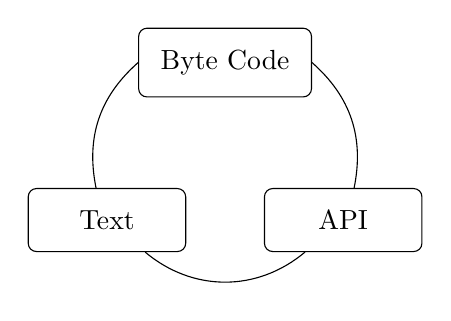
\begin{tikzpicture}[inner sep=2.8mm,
			box/.style={draw,rounded corners=3pt, minimum width=20mm, }]
			\node [box] (bc) at (0, 2) {Byte Code};
			\node [box] (text) at (-1.5, 0) {Text}
				edge[-,bend left=30] (bc.west);
			\node [box] (api) at (1.5,0) {API}
				edge[-,bend left=40] (text)
				edge[-,bend right=30] (bc.east);
		\end{tikzpicture}
	    \caption{Three states of LLVM's IR}
    \end{figure}
  \end{frame}

  \begin{frame}
  	\frametitle{LLVM}
  	\begin{itemize}
  		\item Three-code instructions
  		\item Load/Store
  		\item Infinite number of registers
  	\end{itemize}
  	\begin{block}{SSA in LLVM}
  		As SSA form applies only to registers, the usual way for generating code is to allocate local variables in memory and store results. Optimizer pass will remove unnecessary memory round-trips, generate $\phi$ instructions,  etc...
  	\end{block}
  \end{frame}

\end{document}